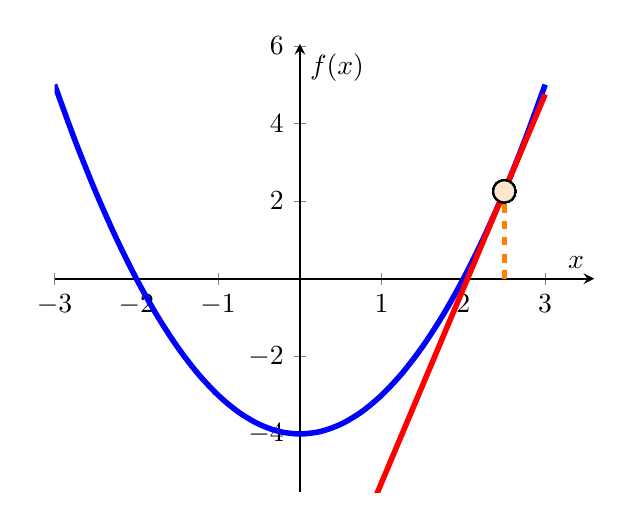
\begin{tikzpicture}
\begin{axis}[axis lines=middle, line width=0.7, enlargelimits=upper, domain=-3:3, ymin=-5.5, xlabel=$x$, ylabel=$f(x)$]
\addplot [smooth, color=blue, line width = 2] {x^2-4};
\addplot[smooth, color=orange, dashed, line width = 2] coordinates {(2.5,0) (2.5,2.25)};
\addplot[only marks, mark size=4, color=orange!20, draw=black] (2.5,2.25);
\addplot [smooth, color=red, line width = 2] {5*x-41/4};
\end{axis}
\end{tikzpicture}